\documentclass{article}


% if you need to pass options to natbib, use, e.g.:
%     \PassOptionsToPackage{numbers, compress}{natbib}
% before loading neurips_2022


% ready for submission
\usepackage[preprint]{neurips_2022}


% to compile a preprint version, e.g., for submission to arXiv, add add the
% [preprint] option:
%     \usepackage[preprint]{neurips_2022}


% to compile a camera-ready version, add the [final] option, e.g.:
%     \usepackage[final]{neurips_2022}


% to avoid loading the natbib package, add option nonatbib:
%    \usepackage[nonatbib]{neurips_2022}


\usepackage[utf8]{inputenc} % allow utf-8 input
\usepackage[T1]{fontenc}    % use 8-bit T1 fonts
\usepackage{hyperref}       % hyperlinks
\usepackage{url}            % simple URL typesetting
\usepackage{booktabs}       % professional-quality tables
\usepackage{amsfonts}       % blackboard math symbols
\usepackage{nicefrac}       % compact symbols for 1/2, etc.
\usepackage{microtype}      % microtypography
\usepackage{xcolor}         % colors

% Felix's packages
\usepackage{amsmath}
\usepackage{amssymb}
\usepackage[shortlabels]{enumitem}
\usepackage{mathtools}
\usepackage{mathrsfs}
\usepackage{dsfont}
\usepackage{physics}
\usepackage{caption}
\usepackage{subcaption}
\usepackage[nameinlink]{cleveref}

% floor, ceiling, set
\DeclarePairedDelimiter{\ceil}{\lceil}{\rceil}
\DeclarePairedDelimiter{\floor}{\lfloor}{\rfloor}
\DeclarePairedDelimiter{\set}{\lbrace}{\rbrace}
\DeclarePairedDelimiter{\iprod}{\langle}{\rangle}
\DeclarePairedDelimiter{\card}{\lvert}{\rvert}
\let\abs\relax
\DeclarePairedDelimiter{\abs}{\lvert}{\rvert}
\DeclarePairedDelimiter{\level}{\llbracket}{\rrbracket}

\DeclareMathOperator{\Int}{int}
\DeclareMathOperator{\bdy}{bdy}
\DeclareMathOperator{\Lim}{Lim}
\DeclareMathOperator{\mean}{mean}
\DeclareMathOperator{\col}{col}
\DeclareMathOperator{\proj}{proj}
\DeclareMathOperator{\dual}{dual}
\usepackage[nameinlink]{cleveref}
\DeclareMathOperator{\opt}{opt}
\DeclareMathOperator{\cone}{cone}
\DeclareMathOperator{\conv}{conv}
\DeclareMathOperator{\supp}{supp}
\DeclareMathOperator{\poly}{poly}
\DeclareMathOperator{\sgn}{sgn}
\DeclareMathOperator{\depth}{depth}
\DeclareMathOperator{\OPT}{OPT}
\DeclareMathOperator{\Set}{set}
\DeclareMathOperator{\pred}{pred}
\DeclareMathOperator{\SAT}{SAT}
\DeclareMathOperator{\indeg}{indeg}
\DeclareMathOperator{\outdeg}{outdeg}
\DeclareMathOperator{\tw}{tw}
\DeclareMathOperator{\bw}{bw}
\DeclareMathOperator{\pw}{pw}
\DeclareMathOperator{\cutwidth}{cutwidth}
\DeclareMathOperator{\Cut}{Cut}
\DeclareMathOperator{\Vs}{Vs}
\DeclareMathOperator{\vs}{vs}
\DeclareMathOperator{\adj}{adj}
\DeclareMathOperator{\Sp}{Sp}
\DeclareMathOperator{\argmax}{argmax}
\DeclareMathOperator{\argmin}{argmin}
\DeclareMathOperator{\dom}{dom}
\DeclareMathOperator{\MLE}{MLE}
\DeclareMathOperator{\MAP}{MAP}
\DeclareMathOperator{\KL}{KL}
\DeclareMathOperator{\LK}{LK}
\DeclareMathOperator{\Be}{Be}
\DeclareMathOperator{\Bin}{Bin}
\DeclareMathOperator{\Geo}{Geo}
\DeclareMathOperator{\Po}{Po}
\DeclareMathOperator{\Exp}{Exp}
\DeclareMathOperator{\Mult}{Mult}
\DeclareMathOperator{\Var}{Var}
\DeclareMathOperator{\Cov}{Cov}
\DeclareMathOperator{\Cauchy}{Cauchy}

% commonly used sets
\newcommand{\R}{\mathbb{R}}
\newcommand{\Z}{\mathbb{Z}}
\newcommand{\N}{\mathbb{N}}
\newcommand{\Q}{\mathbb{Q}}
\newcommand{\C}{\mathbb{C}}
\newcommand{\E}{\mathbb{E}}
\newcommand{\B}{\mathcal{B}}
\newcommand{\F}{\mathcal{F}}
\renewcommand{\L}{\mathcal{L}}
\renewcommand{\P}{\mathbb{P}}

\newcommand{\sset}{\subseteq}
\newcommand{\mcal}{\mathcal}
\newcommand{\mscr}{\mathscr}
\newcommand{\mfrak}{\mathfrak}
\newcommand{\up}{\uparrow}
\newcommand{\down}{\downarrow}
\newcommand{\zeros}{\mathds{0}}
\newcommand{\ones}{\mathds{1}}
\newcommand{\tends}[1]{\xrightarrow{#1}}

\newcommand{\Partition}{{\sc Partition}}

\renewcommand{\bibsection}{}


\title{Weighted Maximum Independent Set Heuristics with Graph Neural Networks}


% The \author macro works with any number of authors. There are two commands
% used to separate the names and addresses of multiple authors: \And and \AND.
%
% Using \And between authors leaves it to LaTeX to determine where to break the
% lines. Using \AND forces a line break at that point. So, if LaTeX puts 3 of 4
% authors names on the first line, and the last on the second line, try using
% \AND instead of \And before the third author name.


\author{%
  Felix Zhou\\
  Department of Computer Science\\
  Yale University\\
  New Haven, CT 06511 \\
  \texttt{felix.zhou@yale.edu} \\
  % examples of more authors
  % \And
  % Coauthor \\
  % Affiliation \\
  % Address \\
  % \texttt{email} \\
  % \AND
  % Coauthor \\
  % Affiliation \\
  % Address \\
  % \texttt{email} \\
  % \And
  % Coauthor \\
  % Affiliation \\
  % Address \\
  % \texttt{email} \\
  % \And
  % Coauthor \\
  % Affiliation \\
  % Address \\
  % \texttt{email} \\
}


\begin{document}


\maketitle


\begin{abstract}
  The weighted maximum indepedent set (WMIS) problem asks us to find a subset of pairwise non-adjacent vertices
  which maximizes the sum of vertex weights.
  In general, there cannot be a constant factor polynomial time approximation algorithm.
  In theory, much progress has been made for solving WMIS for special classes of graphs.
  In practice, exact algorithms based on reduction rules and branching techniques have been examined
  in conjunction with search-based heuristics.
  Graph neural networks (GNNs) have been shown to be effective at learning the structure of real-world graphs.
  Recent efforts have been made to combine simple GNNs with exact methods and iterative search.
  We analyze the performance of different GNN architectures within this paradigm.
  We also provide an easily extensible python implementation of our algorithms for futher exploration.
\end{abstract}


\section{Introduction \& Problem Definition}
Let $G=(V, E)$ be a (simple, undirected) graph with vertex set $V$
and edge set $E$.
Suppose we also have vertex sets $w: V\to \R_{++}$.
Recall that a subset of vertices $I\sset V$ is \emph{independent}
if for every $u\neq v\in I$, $uv\notin E$.
That is, the vertices in $I$ are pairwise non-adjacent.
The weighted maximum independent set problem (WMIS)
asks us to find an independent set $I$ which maximizes $w(I) := \sum_{v\in I} w(v)$.
Note that $I$ is a WMIS in $G$
if and only if $V\setminus I$ is a weighted minimum vertex cover (WMVC) in $G$.
The unweighted decision version of the minimum vertex cover problem (MVC)
was one of Karp's original 21 NP-complete problems.
It follows that both WMVC and WMIS are both NP-hard.
In general graphs,
it is known that the independent set problem (MIS) cannot be approximated within a factor of $n^{1-\epsilon}$ for any $\epsilon > 0$ where $n$ is the number of vertices \citet{zuckerman2006linear}.
In fact, even in 3-regular 3-edge-colorable graphs,
there can be no polynomial time approximation scheme (PTAS) \citet{berman1999appr}.

\section{Dataset}
We consider both real-world graphs and synthetic graphs.
Since these graphs do not come with weights,
we augment each instance with uniformly random integer weights within the interval $[1, N]$.
It is known that with probability at least $1-\frac nN$,
there is a unique solution to WMIS \citet{isolation}.
Thus we chose $N = 2n$ in hopes that this disambiguates supervised learning.

\subsection{PACE 2019 Graphs}
The PACE 2019 competition asked participants to solve MVC in 200 real-world graphs \citet{pace2019}.
Half of the dataset (odd indices) was provided to contestants
and the remaining half (even indices) was used to evaluate submissions.
Solvers were given 30 minutes to solve each instance exactly.
This winning solution by \citet{wegotyoucovered} combined reduction rules,
local search, and a branch and bound scheme.

For each of the 200 graphs, we sampled 100 instances of uniform random weights.
Out of the 10000 instances,  
the state-of-the-art branch and reduce (B\&R) solver by \citet{kamis} solved 18197 cases within 6 hours.

See \Cref{fig:pace} for some elementary statistics about the pace dataset.
It is interesting to note that this dataset is relatively sparse,
with mostly single digit average degree.
Moreover, most graphs have very few connected components.

\begin{figure}
     \centering
     \begin{subfigure}[b]{0.45\textwidth}
         \centering
         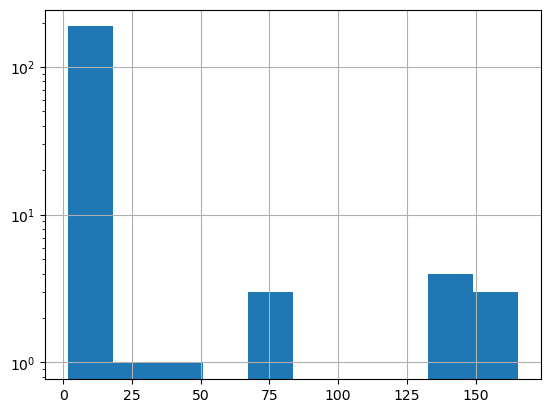
\includegraphics[width=\textwidth]{figures/pace_avg_deg}
         \caption{Average degree of pace graphs.}
         \label{fig:pace_avg_deg}
     \end{subfigure}
     \hfill
     \begin{subfigure}[b]{0.45\textwidth}
         \centering
         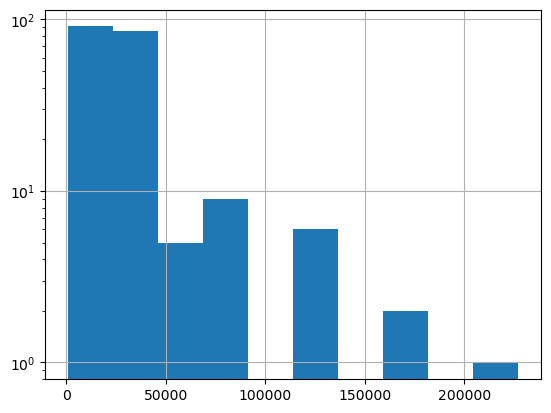
\includegraphics[width=\textwidth]{figures/pace_n_nodes}
         \caption{Number of nodes in pace graphs.}
         \label{fig:pace_n_nodes}
     \end{subfigure}
     
     \bigskip
     \begin{subfigure}[b]{0.45\textwidth}
         \centering
         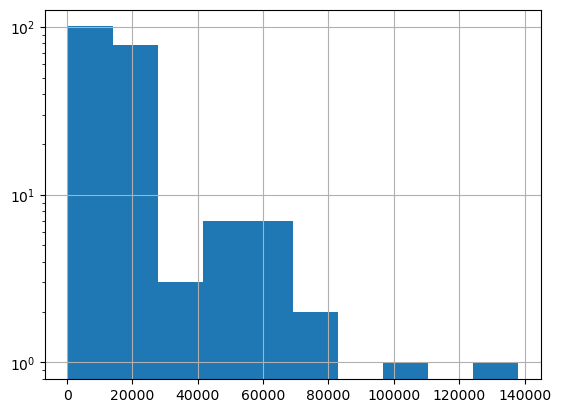
\includegraphics[width=\textwidth]{figures/pace_n_edges}
         \caption{number of edges in pace graphs.}
         \label{fig:pace_n_edges}
     \end{subfigure}
     \hfill
     \begin{subfigure}[b]{0.45\textwidth}
         \centering
         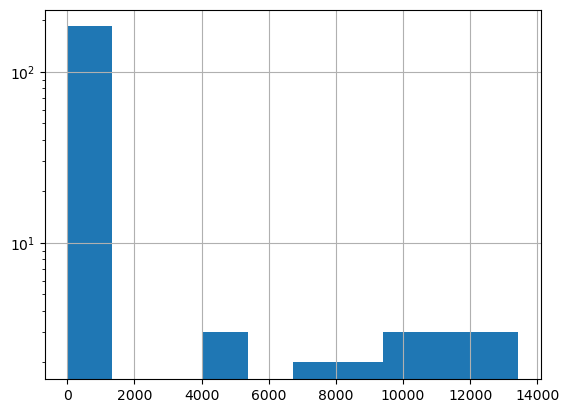
\includegraphics[width=\textwidth]{figures/pace_n_components}
         \caption{Number of components in pace graphs.}
         \label{fig:pace_n_components}
     \end{subfigure}
     \caption{Basic graph statistics as histograms for pace graphs.}
     \label{fig:pace}
\end{figure}

\subsection{Erd\H os-R\'eyni Graphs}
We can generate an instance of an Erd\H os-R\'eyni graph $G(n, p)$ on $n$ vertices
by randomly connecting every pair of vertices independently
with some fixed probability $p$.
Since these are very well-studied graphs,
we omit the graph statistics.

We generated 1000 instaces of $G(200, 0.1)$,
for which the B\&R solver by \citet{kamis} solved all cases within 6 hours.
Next, we generate 5000 instances of $G(1000, 0.005)$,
for which the B\&R solver solved 400 cases within 6 hours.
Finally, we generated 20000 instances of $G(50000, 0.00005)$.
for which the B\&R solver solved all cases within 6 hours.

\subsection{Watts-Strogatz Graphs}
If time permits, we would also like to experiment with Watts-Strogatz graphs $G(n, k, p)$.
Also called ``small-world graphs'',
these graphs are generated by first taking a $k$-regular graph on $n$ vertices
and randomly rewiring each edge with probability $p$.

\section{Description of Related Works}
\subsection{Reductions}
It is helpful to think of WMIS as a 0-1 integer program.
\begin{align*}
  &\max \sum_{v\in V} w(v) x(v) \\
  x(u) + x(v) &\leq 1 &&\forall uv\in E \\
  x &\in \set{0, 1}
\end{align*}
Although we cannot hope to solve 0-1 integer programs polynomial time,
we can relax the integral constraints ($x\in \set{0, 1}^n$)
to form a linear program ($x\in [0, 1]^n$).
Solving this linear program yields a solution $\bar x\in [0, 1]^n$.
It is known that if $\bar x(v) = 1$,
then there is a WMIS which includes $v$
and if $\bar x(v) = 0$,
then there is a WMIS which does not include $v$ \citet{lpreduction}.
Thus we can shrink an instance of WMIS by first solving a linear program
and enforcing that integral vertices are (not) part of the solution.
This is an example of a reduction rule which reduces the sizes of instances
such that any optimal solution for the reduced instance can be expanded to an optimal solution
for the original solution.

Practical solvers for WMIS extensively use reduction rules
in hopes that we can significantly reduce instances
before applying brute force or a heuristic search \cite{kamis}.

\subsection{Graph Neural Networks}
Graph neural networks generalize the concept of convolutions to arbitrary graph-structured data \citet{scarselli2008graph}.
Neural network architectures for graphs have made non-trivial progress on combinatorial optimization problems \citet{cappart2021combinatorial}.
For example, we can consult a graph convolutional network (GCN) as part of an iterative search,
whether some vertex is part of some optimal solution \citet{comboptgcn}.
The authors referred this as a \emph{reducing-peeling} strategy.

Following this line of works,
\citet{langedal_et_al} combined techniques from exact methods,
iterative search,
and GNNs.
The authors first compute a greedy solution using reduction rules when possible.
Then, a simple 3-layer GNN is applied to select a vertex likely to be in or out of the solution,
potentially opening up for further reductions.
Finally, a local search strategy is used to enhance the solution.
They also provided a C++ implementation
and conducted experiments on some SuiteSparse graphs \citet{suitesparse}.
However, we were unable to obtain the exact dataset used.

\section{Proposed Approaches}
Our approach can be summarize by the following:
\begin{enumerate}[1)]
  \item Compute reductions (optional).
  \item Consult GNN as in reducing-peeling.
  \item Go to 1) (optional).
  \item Compute a final feasible solution.
\end{enumerate}
Our overall goal is two-fold.
First, we would like to build on the framework of \citet{langedal_et_al}
with a focus on the architecture of the GNN employed
and less attention on the reductions and local search techniques.
Secondly, we would like to provide a highly extensible framework in Python3
which faciliates further experimentation.

\subsection{Computing Reductions (Optional)}
Before consulting our GNN,
we can optionally apply some reduction rules.
We will leverage the popular LP solver Gurobi \citet{gurobi}
and implement the LP reduction by \citet{lpreduction}.

\subsection{GNN Architecture}
We will begin with the 3-layer GNN architecture from \citet{langedal_et_al}
implemented in PyTorch Geometric \citet{pyg},
a library built upon the popular PyTorch framework \citet{pytorch}.
Next, we would like to experiment with more expressive architectures
such as Identity-Aware GNNs by \citet{idgnn}.
The output of our GNN should be a value between $[0, 1]$ for every node
which we interpret as the likelihood of that node belonging to an optimal solution.

\subsection{Iterating (Optional)}
Given the output from our GNN,
we can optionally attempt further reductions before computing a final solution.

\subsection{Computing a Final Solution}
If the current solution is not integral,
there is a simple greedy algorithm to ``round'' the solution to an independent.
Namely, we sort the vertices in non-increasing fashion based on the value in the current solution.
Then, we greedily add the highest unprocessed vertex to our independent set
while marking all of this neighbors as not belonging to the set.

\section{Evaluation Metrics}
We would like to evaluate the performance of our framework on the PACE 2019 dataset \citet{pace2019},
Erd\H os-R\'eyni graphs,
and Watts-Strogatz graphs (if time permits) in two ways.
we would first like to look at the approximation ratio of our algorithm compared to the exact solutions
computed using B\&R \citet{kamis}.
Then, we would like to compare the approximation ratio of our algorithms compared to a heuristic local search
restricted to 30 minutes B\&R.
The second metric is necessary since the exact solver was unable to find the optimal result for about 10\% of graphs.

On the PACE 2019 dataset,
we will imitate the conditions of the contest and train our models on the odd-indexed graphs.
For the random graphs,
we will reserve 20\% of the labeled dataset for evaluation
and the rest for training.

If time permits,
it would be interesting to plot the approximation ratio (compared to the exact solution)
against the parameters of random graphs.
For instance, the $k$ parameter of the Watts-Strogatz graphs $G(n, k, p)$
and the $p$ parameter of the Erd\H os-R\'eyni graphs $G(n, p)$.

\section{Timeline}
We plan on spending one week on each of the following tasks:
\begin{enumerate}[(i)]
  \item Implement LP reduction and final greedy algorithm.
  \item Implement basic 3-layer GNN and identity-aware GNN.
  \item Train and evaluate on PACE 2019 graphs.
  \item Train and evaluate on Erd\H os-R\'eyni graphs.
  \item Iterate on GNN architecture.
  \item Train and evaluate on PACE 2019 and Erd\H os-R\'eyni graphs.
  \item Train and evaluate on Watts-Strogatz graphs (if time permits).
\end{enumerate}

\section{References}
\bibliographystyle{plainnat}
\bibliography{proposal.bib}


\end{document}
